\documentclass[conference]{IEEEtran}

\usepackage{amsmath}
\usepackage{amssymb}
\usepackage{booktabs}
\usepackage{array}
\usepackage{graphicx}
\usepackage{multirow}
\usepackage{subcaption}
\usepackage[hidelinks]{hyperref}

\graphicspath{{figures/}}

\title{Comparative Evaluation of Methods for Position-Independent\\
Voiced-Consonant Detection in Isolated Words}

\author{\IEEEauthorblockN{Bunyod Suvonov and Giorgio Aman Soetomo}}

\begin{document}

\maketitle

\begin{abstract}
This paper presents a comparative evaluation of methods for position-independent full-word detection of four voiced consonants, \textit{d}, \textit{n}, \textit{r}, and \textit{v}, using recordings from Speech Commands v0.02. The target consonant may appear at the beginning, middle, or end of the word, so the detection problem is formulated as letter presence over the whole active word. A 19-keyword benchmark is constructed so that each target consonant has exactly four positive keyword types while the targets still occur in initial, medial, and final positions across the benchmark. We compare five classical detectors and one multilayer perceptron (MLP) baseline: global fast Fourier transform (FFT) template matching, Mel-frequency cepstral coefficient (MFCC) mean-template scanning, MFCC + dynamic time warping (DTW), local short-time Fourier transform (STFT) mean-template scanning, local STFT $k$-nearest-neighbor (k-NN) scanning, and a small MLP operating on full-word log-Mel features. The FFT/STFT spectrum detectors are implemented in MATLAB, while the MFCC/DTW and MLP detectors provide comparison methods from speech recognition and neural-network modeling. On balanced speaker-independent test sets, the classical methods achieve macro F1 between 66.18\% and 67.85\%, while the MLP reaches 86.25\% macro F1 and 86.46\% macro accuracy. In these experiments, coarse template detectors have high recall but poor precision under word-level labels and weak phoneme alignment, whereas the trained MLP gives a sharper full-word decision boundary.
\end{abstract}

\section{Introduction}
Speech is a time-domain waveform, but many phonetic cues become much clearer after short-time spectral analysis. Sampling, Fourier analysis, and local spectra make physically meaningful structure visible. This work uses those tools as part of a controlled comparison of detectors for deciding whether selected voiced consonants are present in spoken isolated words. Speech Commands v0.02 is a public corpus of short, single-word speech recordings designed for limited-vocabulary keyword-spotting research; here it is used as a source of isolated-word utterances with word labels.

The critical methodological issue is \emph{position}. A target consonant can occur in different parts of an isolated word, for example \textit{d} in \textit{dog} and \textit{bed}, or \textit{r} in \textit{right} and \textit{zero}. Therefore, we study position-independent detection of four voiced consonants:
\begin{itemize}
    \item \textit{d}: voiced alveolar stop,
    \item \textit{n}: voiced nasal stop,
    \item \textit{r}: voiced liquid,
    \item \textit{v}: voiced labiodental fricative.
\end{itemize}

The comparative study is organized around three questions:
\begin{enumerate}
    \item How can local spectral templates be extracted for consonants in word-level recordings?
    \item How well do classical spectrum, Mel-frequency cepstral coefficient (MFCC), and dynamic time warping (DTW) detectors work when the target consonant may occur anywhere in the word?
    \item How does a multilayer perceptron (MLP) classifier trained directly on whole-word features compare with the classical detectors?
\end{enumerate}

The contribution is a controlled comparison of six detectors on the same 19-keyword Speech Commands benchmark, with identical letter labels, speaker-independent splits, and metrics. Local target templates are constructed from approximate phoneme-position priors, and each local detector scans the entire active part of the word at test time.

\section{Related Work}
Classical speech recognition relied heavily on short-time spectral analysis and template matching. Rabiner and Schafer describe the central role of short-time processing in speech analysis~\cite{rabiner1978digital}. Davis and Mermelstein introduced MFCCs as a compact and effective spectral representation for speech recognition~\cite{davis1980comparison}. Sakoe and Chiba proposed DTW to align speech templates under speaking-rate variability~\cite{sakoe1978dynamic}. These ideas motivate the MFCC and DTW baselines used here.

Modern speech systems increasingly use learned models rather than direct template matching. Hinton \textit{et al.} summarized the impact of deep neural networks on acoustic modeling~\cite{hinton2012dnn}. For limited-vocabulary speech tasks, Sainath and Parada showed that compact neural networks can outperform conventional baselines in keyword spotting~\cite{sainath2015cnn}. Speech Commands was introduced by Warden as a public benchmark for limited-vocabulary keyword spotting and has been widely used to evaluate isolated-word speech recognition methods~\cite{warden2018speech}.

Our comparison therefore includes MATLAB spectrum methods based on the fast Fourier transform (FFT) and short-time Fourier transform (STFT), MFCC/DTW baselines, and an MLP trained on the same Speech Commands recordings.

\section{Problem Formulation and Theory}
\subsection{Sliding-Window Letter Detection}
Let $x[n]$ be a word recording and let $[t_s,t_e]$ denote its active speech region after simple energy-based voice activity detection. We slide a fixed analysis window across that active region and obtain local segments
\begin{equation}
w_m[n] = x[n+t_m], \quad m=1,\dots,M.
\end{equation}
For a target consonant $c$, a template bank $B_c=\{b_{c,1},\dots,b_{c,K_c}\}$ is built from training recordings. A generic scan detector uses
\begin{equation}
S_c(x)=\max_m g_c(\phi(w_m),B_c),
\end{equation}
where $\phi(\cdot)$ is the chosen local feature map and $g_c$ is the method-dependent bank score: maximum cosine similarity, negative DTW distance, or top-$k$ average cosine similarity. The final decision is
\begin{equation}
\hat{y}_c(x)=
\begin{cases}
1, & S_c(x)\ge \tau_c,\\
0, & S_c(x)< \tau_c,
\end{cases}
\end{equation}
with threshold $\tau_c$ chosen on the validation set.

\subsection{Approximate Phoneme-Position Prior}
Speech Commands provides word labels but not phoneme boundaries. To initialize target templates, we map each selected keyword to a simple ARPABET (ARPA phonetic alphabet) pronunciation and approximate the target-phoneme center by a uniform partition of the active word. If a word has $L$ phonemes and the target occurs at zero-based phoneme index $i$, we estimate its center as
\begin{equation}
\hat{t}_i=t_s+\frac{i+0.5}{L}(t_e-t_s).
\end{equation}
This weak alignment assumption is used only during training to choose template windows. Word labels are also used to define positive and negative examples and to compute ground-truth evaluation metrics. They are not used as inputs to the detector at test time: the detector receives only the waveform-derived spectral features and then scans the whole active region.

\subsection{Short-Time Spectrum, MFCC, and DTW}
For a frame window $h[n]$, the short-time Fourier transform (STFT) is
\begin{equation}
X_{w,r}[k]=\sum_{n=0}^{N-1} w[n+rH] h[n] e^{-j2\pi kn/N}.
\end{equation}
For each scanned 100~ms analysis window, the local STFT feature is constructed by computing the log-magnitude STFT inside that window and then averaging over its short-time frames:
\begin{equation}
\phi_{\mathrm{STFT}}(w)[k]=\frac{1}{M_w}\sum_{r=1}^{M_w}\log\left(|X_{w,r}[k]|+\epsilon\right).
\end{equation}
Thus $\phi_{\mathrm{STFT}}(w)$ is a single spectrum vector describing the local frequency content of one consonant-sized region of the word. The local STFT detectors compare this vector with target-consonant templates using cosine similarity. This keeps the detector directly interpretable in the frequency domain.

Mel-frequency cepstral coefficients (MFCCs) compress the short-time spectrum into a perceptually motivated cepstral representation. If $E_m[b]$ is the Mel-band energy of frame $m$ and band $b$, then
\begin{equation}
c_m[q]=\sum_{b=0}^{B-1} \log E_m[b]\cos\!\left(\frac{\pi(b+1/2)q}{B}\right).
\end{equation}
Dynamic time warping (DTW) then compares two MFCC sequences by the minimum dynamic-programming path cost under local step constraints~\cite{sakoe1978dynamic}. In our detector, DTW is applied between every scanned test window and a small bank of representative target templates.

\subsection{MLP Detector}
For the multilayer perceptron (MLP) method, each full word is converted into a resized log-Mel spectrogram vector $z(x)$. We train one binary MLP per target consonant:
\begin{equation}
p_c(x)=\sigma\!\left(W_2 \rho(W_1 \tilde{z}(x)+b_1)+b_2\right),
\end{equation}
where $\tilde{z}(x)$ is standardized, $\rho(\cdot)$ is the rectified linear unit (ReLU), and $\sigma(\cdot)$ is the sigmoid function. This model sees the entire word at once and is not limited to one local template.

\section{Dataset and Experimental Setup}
\subsection{Dataset and Target Selection}
We use the full Speech Commands v0.02 dataset~\cite{warden2018speech}. From it, we select 19 keywords:
\textit{backward}, \textit{bed}, \textit{bird}, \textit{cat}, \textit{dog}, \textit{five}, \textit{four}, \textit{go}, \textit{house}, \textit{marvin}, \textit{no}, \textit{on}, \textit{right}, \textit{seven}, \textit{up}, \textit{visual}, \textit{wow}, \textit{yes}, and \textit{zero}.
Six of these keywords, \textit{cat}, \textit{go}, \textit{house}, \textit{up}, \textit{wow}, and \textit{yes}, do not contain any of the four target consonants and are included as target-free negative examples. To keep the computation comparable across all methods, each keyword is capped at 150 training recordings, 60 validation recordings, and 120 test recordings, giving 6,270 recordings in total.

The split is speaker-independent. In Speech Commands filenames such as \texttt{00b01445\_nohash\_0.wav}, the token before \texttt{\_nohash\_} is a hexadecimal speaker identifier. We convert this token to an integer and then take modulo 100, which maps each speaker to a deterministic bucket from 0 to 99. Buckets 0--19 are assigned to the test set, buckets 20--29 to the validation set, and buckets 30--99 to the training set. Thus the split is approximately 70\%/10\%/20\% train/validation/test by speaker before the per-keyword caps are applied. This is different from a random 80\%/20\% utterance split: every recording from the same speaker goes to the same partition, which avoids evaluating on the same speaker identities seen during training.

Table~\ref{tab:targets} shows the positive keywords for each target consonant. The labels I/M/F denote initial, medial, and final target positions in the approximate pronunciation. The positive keyword design is lexically balanced: each target consonant appears in exactly four selected keyword types. Some words contain more than one target consonant, so they can be positive examples for more than one binary detector.

\begin{table*}[t]
    \centering
    \caption{Target consonants, phonetic roles, and positive keyword set used in the experiments}
    \label{tab:targets}
    \begin{tabular}{p{1.2cm}p{3.0cm}p{11.2cm}}
        \toprule
        Target & Phonetic role & Positive keywords used for detection \\
        \midrule
        \textit{d} & voiced alveolar stop & \textit{backward}(F), \textit{bed}(F), \textit{bird}(F), \textit{dog}(I) \\
        \textit{n} & voiced nasal stop & \textit{marvin}(F), \textit{no}(I), \textit{on}(F), \textit{seven}(F) \\
        \textit{r} & voiced liquid & \textit{four}(F), \textit{marvin}(M), \textit{right}(I), \textit{zero}(M) \\
        \textit{v} & voiced labiodental fricative & \textit{five}(F), \textit{marvin}(M), \textit{seven}(M), \textit{visual}(I) \\
        \bottomrule
    \end{tabular}
\end{table*}

For each target consonant, the word label is converted into a binary presence label using the pronunciation table. For example, \textit{marvin} is positive for \textit{n}, \textit{r}, and \textit{v}, but negative for \textit{d}. The negative class is sampled from the remaining selected keywords that do not contain that target. The negative examples are subsampled to match the number of positive examples, so every detection problem is balanced. During testing, these labels are used only to score the predictions, not to generate them.

\subsection{Assumptions and Preprocessing}
The experiments use the following assumptions:
\begin{itemize}
    \item Speech Commands provides word labels but not phoneme boundaries.
    \item Active speech can be isolated by an energy threshold on 20~ms frames with 10~ms hop.
    \item Approximate phoneme timing can be estimated by dividing the active region according to pronunciation length.
    \item Detection is position-independent at test time, so all local methods scan the full active word.
\end{itemize}

Each recording is mean-removed and peak-normalized. The active region is then detected by thresholding short-time energy at 10\% of the utterance maximum. Local detectors use a 100~ms analysis window, a 25~ms STFT frame, 10~ms hop, and 512-point FFT. MFCC features use 26 Mel filters and 13 cepstral coefficients.

\subsection{Implemented Methods}
We compare six methods. The global FFT, local STFT mean-template, and local STFT $k$-nearest-neighbor (k-NN) detectors form the MATLAB spectrum-based implementation. MFCC mean-template and MFCC + DTW are speech-recognition baselines, and the MLP is trained for the same detection task. The MLP is included as a learned whole-word baseline, not as an a priori preferred method; all methods use the same train/validation/test protocol. Table~\ref{tab:structures} summarizes the models, assumptions, and decision rules.

Figure~\ref{fig:methodmap} connects the method names to the algorithmic blocks. A \emph{method} is a concrete feature and scoring choice, while an \emph{algorithm block} is a reusable procedure. Thus, four local template methods share the same template-building and full-word scanning structure, while differing in feature representation and similarity score.

\begin{figure}[t]
    \centering
    \small
    \setlength{\fboxsep}{4pt}
    \fbox{\parbox{0.88\linewidth}{\centering Input: one isolated-word waveform}}\\[1mm]
    $\downarrow$\\[-1mm]
    \fbox{\parbox{0.88\linewidth}{\centering \textbf{Algorithm 1: common preprocessing}\\mean removal, peak normalization, active-speech detection, full-word features, and local scanning windows}}\\[1mm]
    $\downarrow$\\[-1mm]
    \emph{Choose one method branch}\\[1mm]
    \fbox{\parbox{0.88\linewidth}{\textbf{A. Whole-word template}\\Method: global FFT template. Train one positive whole-word spectrum template per target; test by cosine similarity and validation-tuned threshold.}}\\[1mm]
    \fbox{\parbox{0.88\linewidth}{\textbf{B. Local template scan}\\Algorithms 2--3. Methods: MFCC mean-template, MFCC + DTW, local STFT mean-template, and local STFT k-NN. Train target-window template banks; test by scanning all active-word windows and thresholding the best score.}}\\[1mm]
    \fbox{\parbox{0.88\linewidth}{\textbf{C. Learned full-word classifier}\\Algorithm 4. Method: MLP classifier. Train one binary network on full-word log-Mel features; test by thresholding the output probability.}}
    \caption{Block diagram linking the six implemented methods to the four shared algorithm structures. Algorithm 2 builds classical templates and Algorithm 3 scores test recordings.}
    \label{fig:methodmap}
\end{figure}

\begin{table*}[t]
    \centering
    \caption{Implemented methods, feature spaces, assumptions, and decision rules}
    \label{tab:structures}
    \begin{tabular}{p{2.4cm}p{3.2cm}p{4.7cm}p{5.1cm}}
        \toprule
        Method & Feature / model & Training assumptions and structure & Test-time decision rule \\
        \midrule
        Global FFT template & Whole active-word log FFT spectrum & Build one positive mean template per letter from whole-word spectra; threshold tuned on validation set & Detect the letter if cosine similarity to the positive template exceeds the tuned threshold \\
        MFCC mean-template scan & 13-dimensional MFCC mean of each 100~ms local window & Use pronunciation-based target windows to form initial/medial/final positive template means & Scan the active word and take the maximum cosine similarity over all windows and templates \\
        MFCC + DTW & Sequence of MFCC vectors inside each 100~ms local window & Use pronunciation-based target windows to form a representative positive bank; tune template count and Sakoe--Chiba band on validation data & Scan the active word and use the negative minimum DTW distance as the score \\
        Local STFT mean-template scan & Average local log spectrum of each 100~ms window & Use pronunciation-based target windows to form initial/medial/final positive spectral templates & Scan the active word and take the maximum cosine similarity over all windows and templates \\
        Local STFT k-NN scan & Bank of local average log spectra & Store representative target windows; tune $k$ on validation data & Scan the active word and use the best top-$k$ average cosine similarity as the score \\
        MLP classifier & Whole-word resized log-Mel spectrogram vector & Train one binary MLP per letter with ReLU, sigmoid output, Adam, and early stopping & Use the output probability and a validation-tuned threshold to decide letter presence \\
        \bottomrule
    \end{tabular}
\end{table*}

\subsection{Algorithm Structure}
The algorithmic structure is summarized in Fig.~\ref{fig:methodmap}. Algorithm~1 is common preprocessing: waveform normalization, active-speech detection, and generation of both full-word features and local scanning windows. This block is shared by all six methods.

Algorithm~2 builds classical templates. For the global FFT method, the positive training recordings are represented by whole-word log spectra and averaged to form one target template. For the local methods, positive words are first mapped to their pronunciation strings, the approximate target position is estimated using (4), and the closest 100~ms local window is extracted. The selected local windows form either mean templates, representative DTW templates, or a k-NN template bank.

Algorithm~3 scores classical test recordings. The global FFT branch computes one cosine similarity score between the test word and the target template. The local branches scan all active-word windows and keep the best target score over time. The score is maximum cosine similarity for mean-template matching, negative minimum DTW distance for MFCC + DTW, and best top-$k$ average cosine similarity for local STFT k-NN. In all cases, the final threshold is selected on the validation set.

Algorithm~4 is the MLP branch. It converts the active word into a resized full-word log-Mel vector, standardizes it using training-set statistics, trains one binary MLP per target consonant, and uses a validation-tuned probability threshold for the final decision.

\section{Spectral Analysis}
Figure~\ref{fig:spectra} shows the average local spectra extracted from the estimated target windows. Even with weak phoneme alignment, the targets remain distinguishable. The stop consonant \textit{d} shows a short transition-like spectrum, \textit{n} concentrates more low-frequency energy because of nasal resonance, \textit{r} has a smoother vowel-like transition, and \textit{v} contributes frication energy from a voiced labiodental constriction.

Figure~\ref{fig:examples} validates the task definition by showing highlighted windows at different target positions: \textit{d} is captured at the end of \textit{bed}, \textit{n} at the end of \textit{seven}, \textit{r} in the middle of \textit{zero}, and \textit{v} at the beginning of \textit{visual}. These examples illustrate the full-word scanning problem.

\begin{figure}[t]
    \centering
    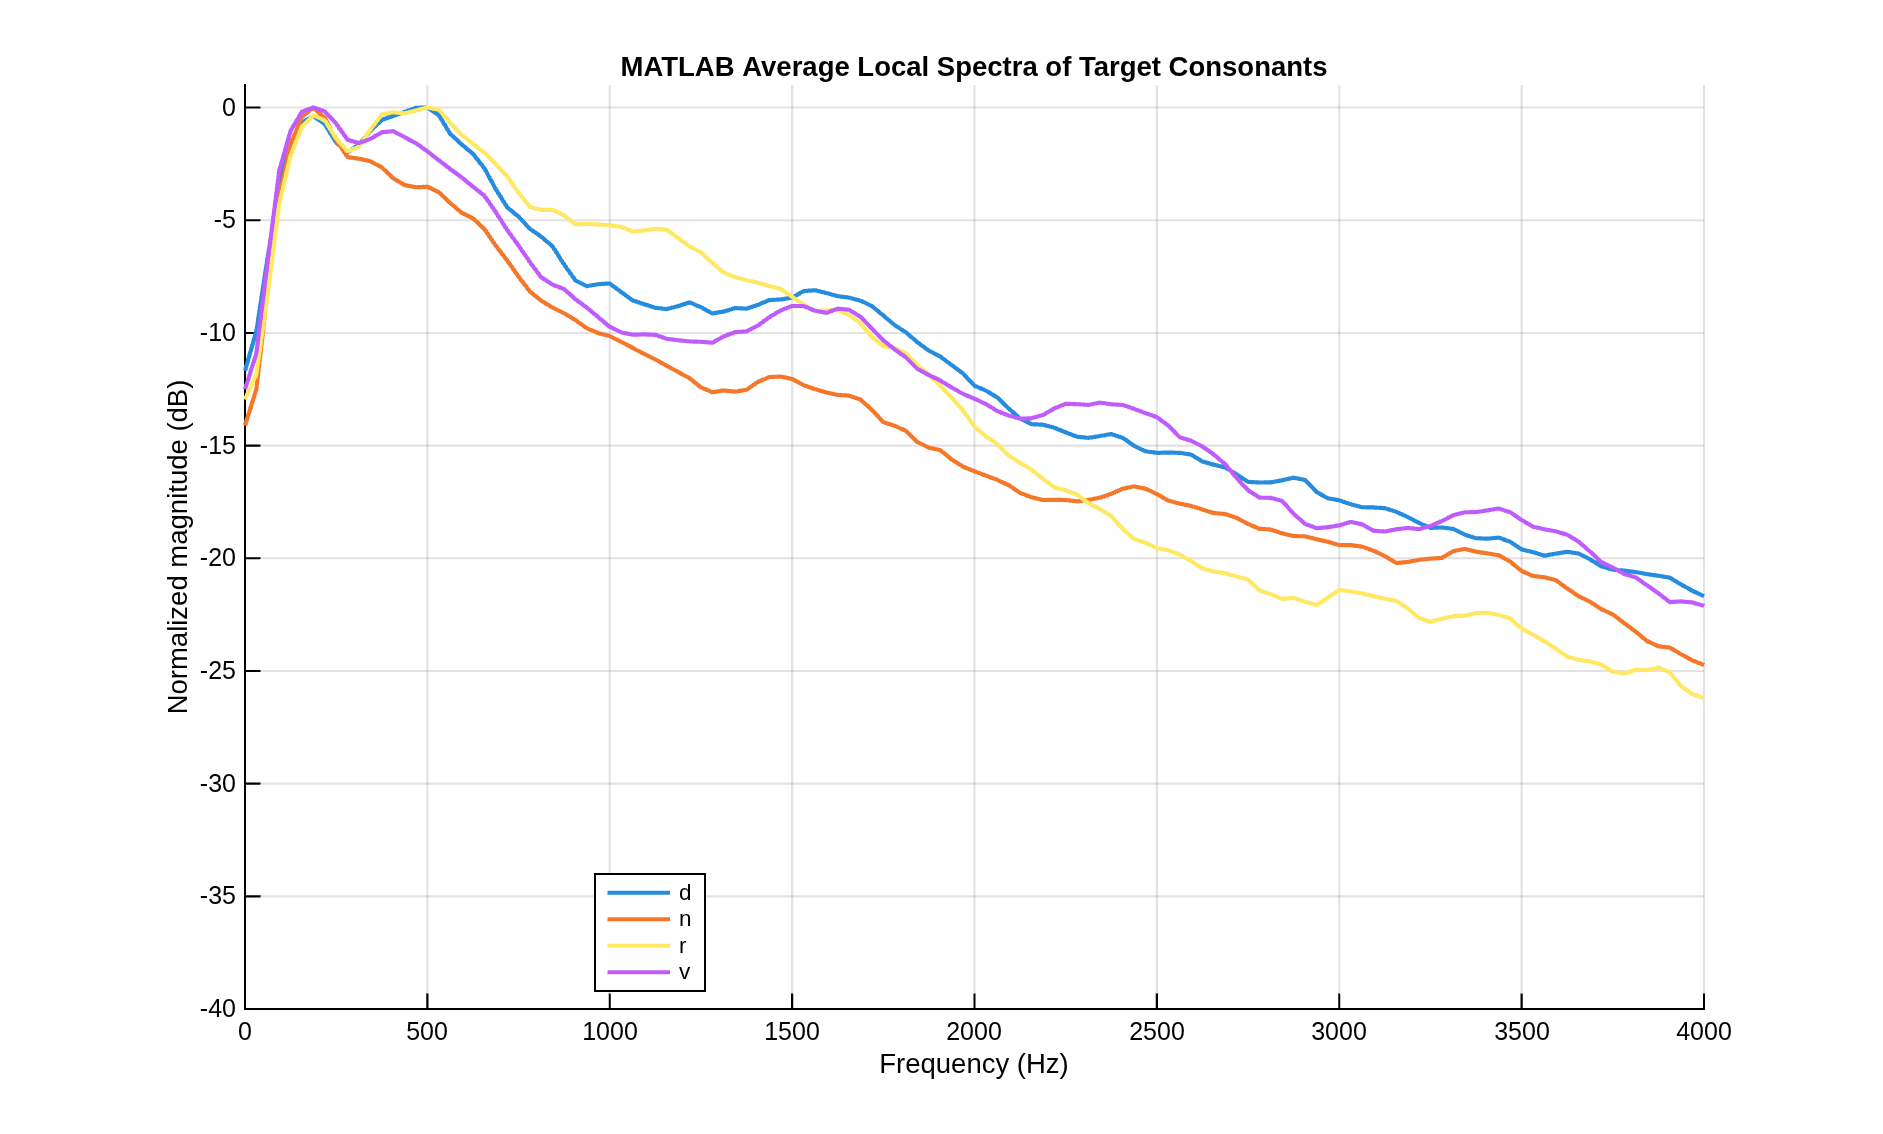
\includegraphics[width=\linewidth]{matlab_fullword_average_local_spectra.png}
    \caption{MATLAB average local spectra of the four voiced consonants extracted from approximate target windows.}
    \label{fig:spectra}
\end{figure}

\begin{figure}[t]
    \centering
    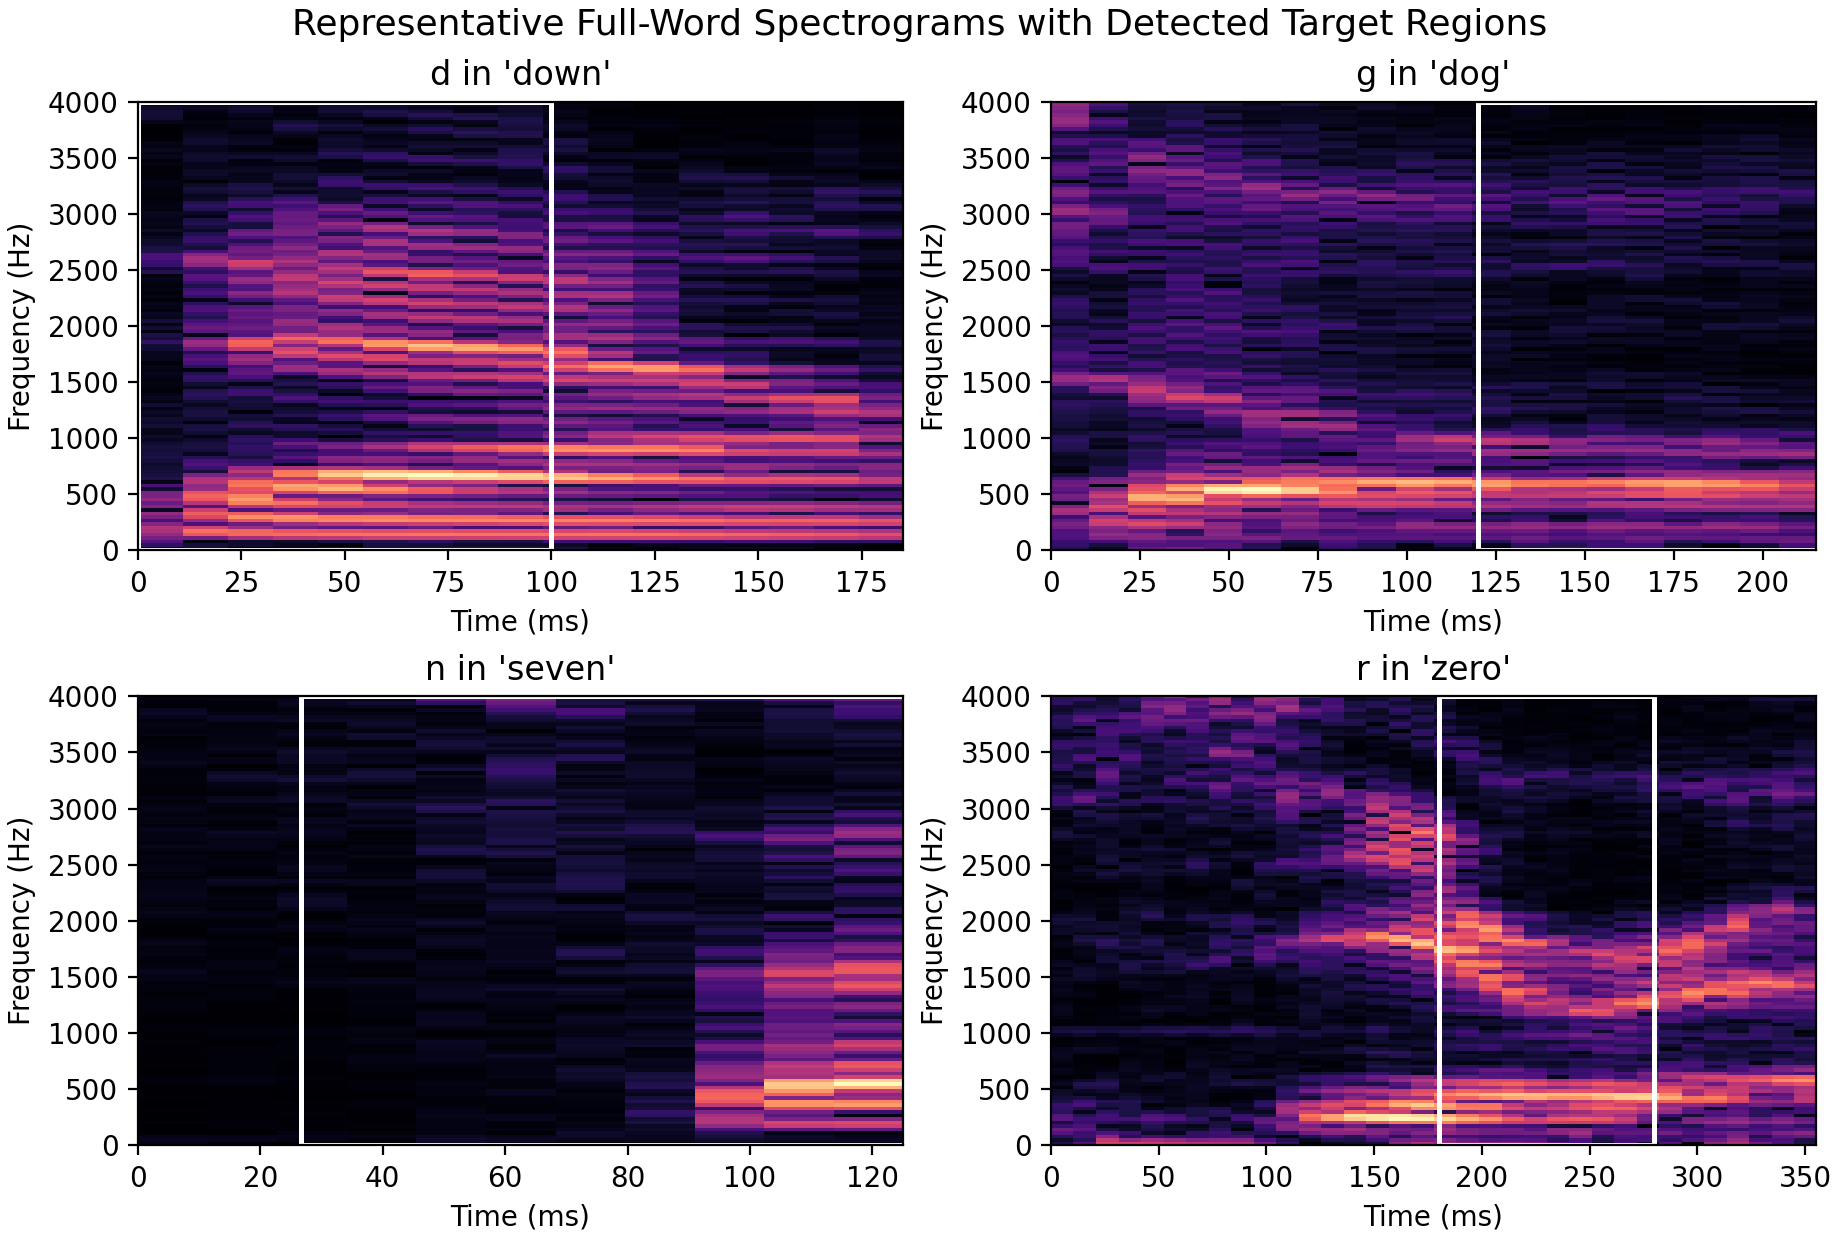
\includegraphics[width=\linewidth]{fullword_position_examples.png}
    \caption{Representative full-word spectrograms with highlighted target windows. The examples include initial, final, and medial consonant positions.}
    \label{fig:examples}
\end{figure}

\section{Results and Comparisons}
\subsection{Overall Comparison}
Table~\ref{tab:overall} reports the average precision, recall, F1, and accuracy over the four balanced binary detection tasks. The average metrics show that the classical detectors are recall-heavy but imprecise, while the MLP gives more balanced precision and recall.

\begin{table*}[t]
    \centering
    \caption{Average detection performance across the four target consonants on the speaker-independent test split}
    \label{tab:overall}
    \begin{tabular}{lcccc}
        \toprule
        Method & Macro precision (\%) & Macro recall (\%) & Macro F1 (\%) & Macro accuracy (\%) \\
        \midrule
        Global FFT template & 50.38 & 99.22 & 66.82 & 50.73 \\
        MFCC mean-template scan & 53.12 & 94.64 & 67.85 & 55.03 \\
        MFCC + DTW & 51.18 & 96.04 & 66.72 & 52.08 \\
        Local STFT mean-template scan & 51.82 & 94.11 & 66.65 & 52.92 \\
        Local STFT k-NN scan & 51.87 & 91.82 & 66.18 & 53.15 \\
        MLP classifier & 86.87 & 86.04 & 86.25 & 86.46 \\
        \bottomrule
    \end{tabular}
\end{table*}

The MATLAB spectrum implementation was also run separately for the FFT/STFT detectors. It gave comparable macro F1 values: 66.65\% for global FFT, 66.02\% for local STFT mean-template scanning, and 65.93\% for local STFT k-NN scanning. These values agree with Table~\ref{tab:overall}: classical spectrum scanning is useful for spectral interpretation, but in this benchmark it is less selective than the MLP under weak phoneme alignment.

Figure~\ref{fig:overallfig} presents the same comparison graphically. The five classical methods cluster closely together because they all depend on weakly aligned target templates. Once the target is allowed to occur anywhere in the word, coarse positive-template scanning becomes difficult to make selective.

\begin{figure}[t]
    \centering
    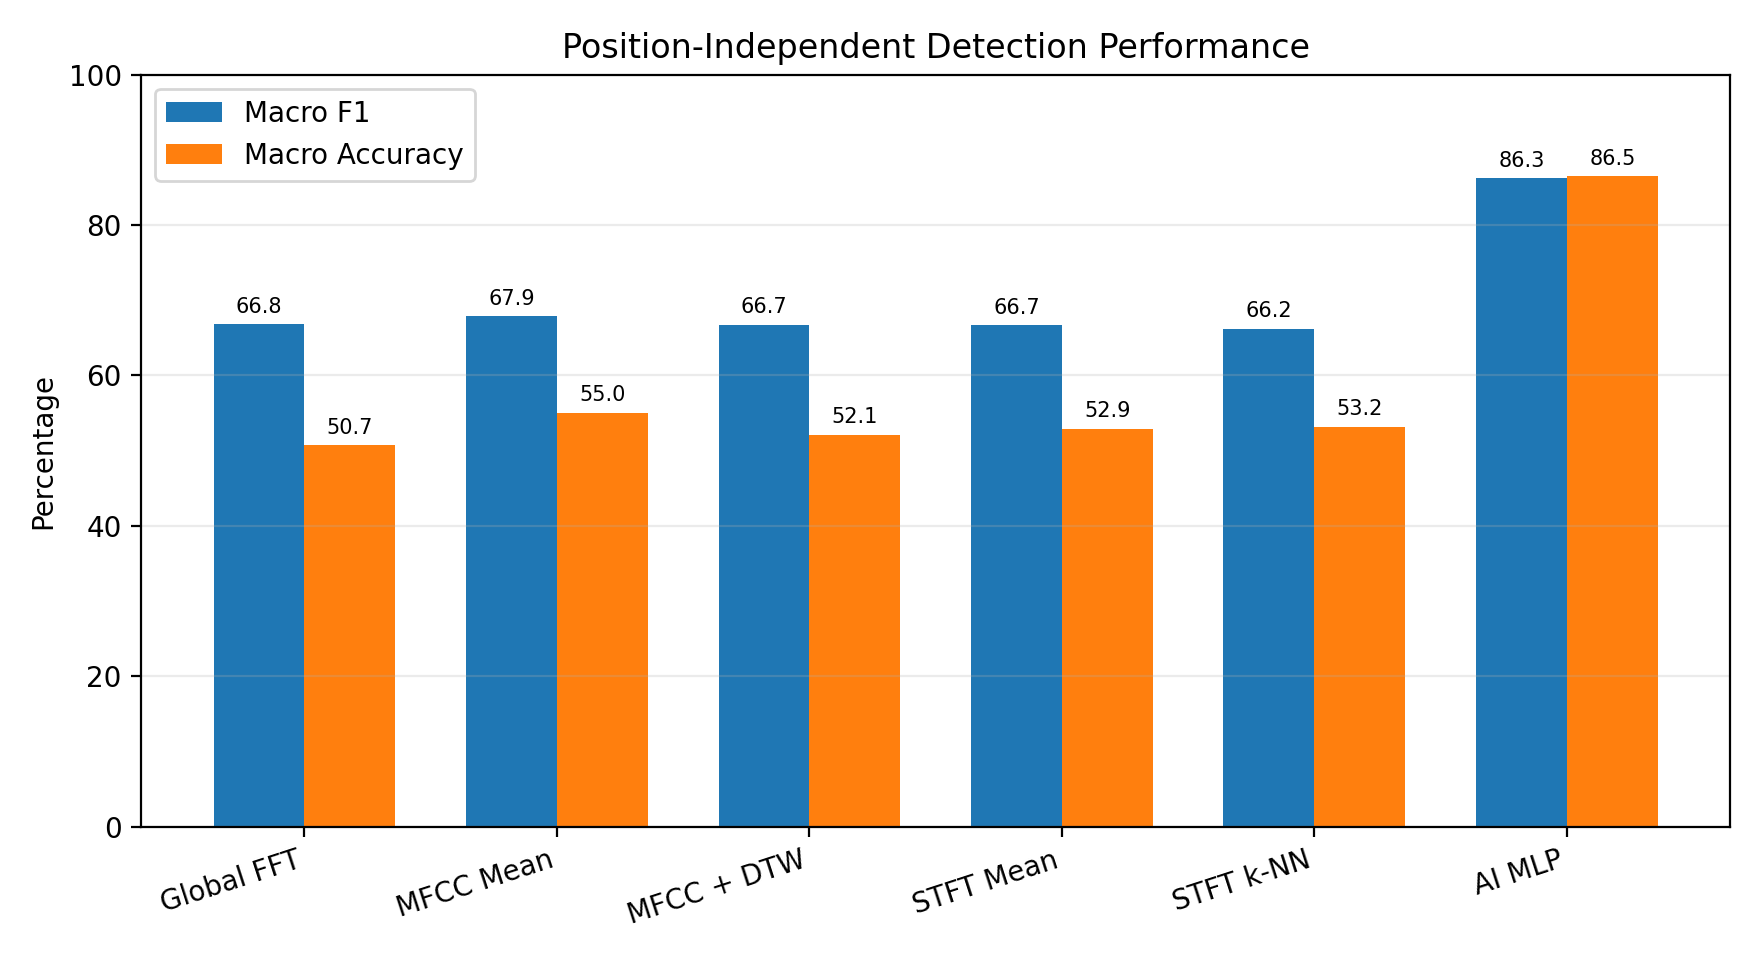
\includegraphics[width=\linewidth]{fullword_method_comparison.png}
    \caption{Macro F1 and macro accuracy for all implemented methods. Percentage labels are printed above the bars to make close classical baseline values readable.}
    \label{fig:overallfig}
\end{figure}

\subsection{Per-Letter Comparison}
Figure~\ref{fig:perletter} compares one MFCC/DTW baseline, one local-spectrum classical detector (STFT k-NN), and the MLP on each letter. In the test results, the MLP obtains the highest F1 for all four consonants: 86.39\% for \textit{d}, 80.63\% for \textit{n}, 88.98\% for \textit{r}, and 89.00\% for \textit{v}.

Among the classical methods, performance is especially limited for letters whose target windows are hard to isolate with only word-level supervision. This is expected: the classical detectors know how the target should look locally, but they do not learn a global representation of the entire word.

\begin{figure}[t]
    \centering
    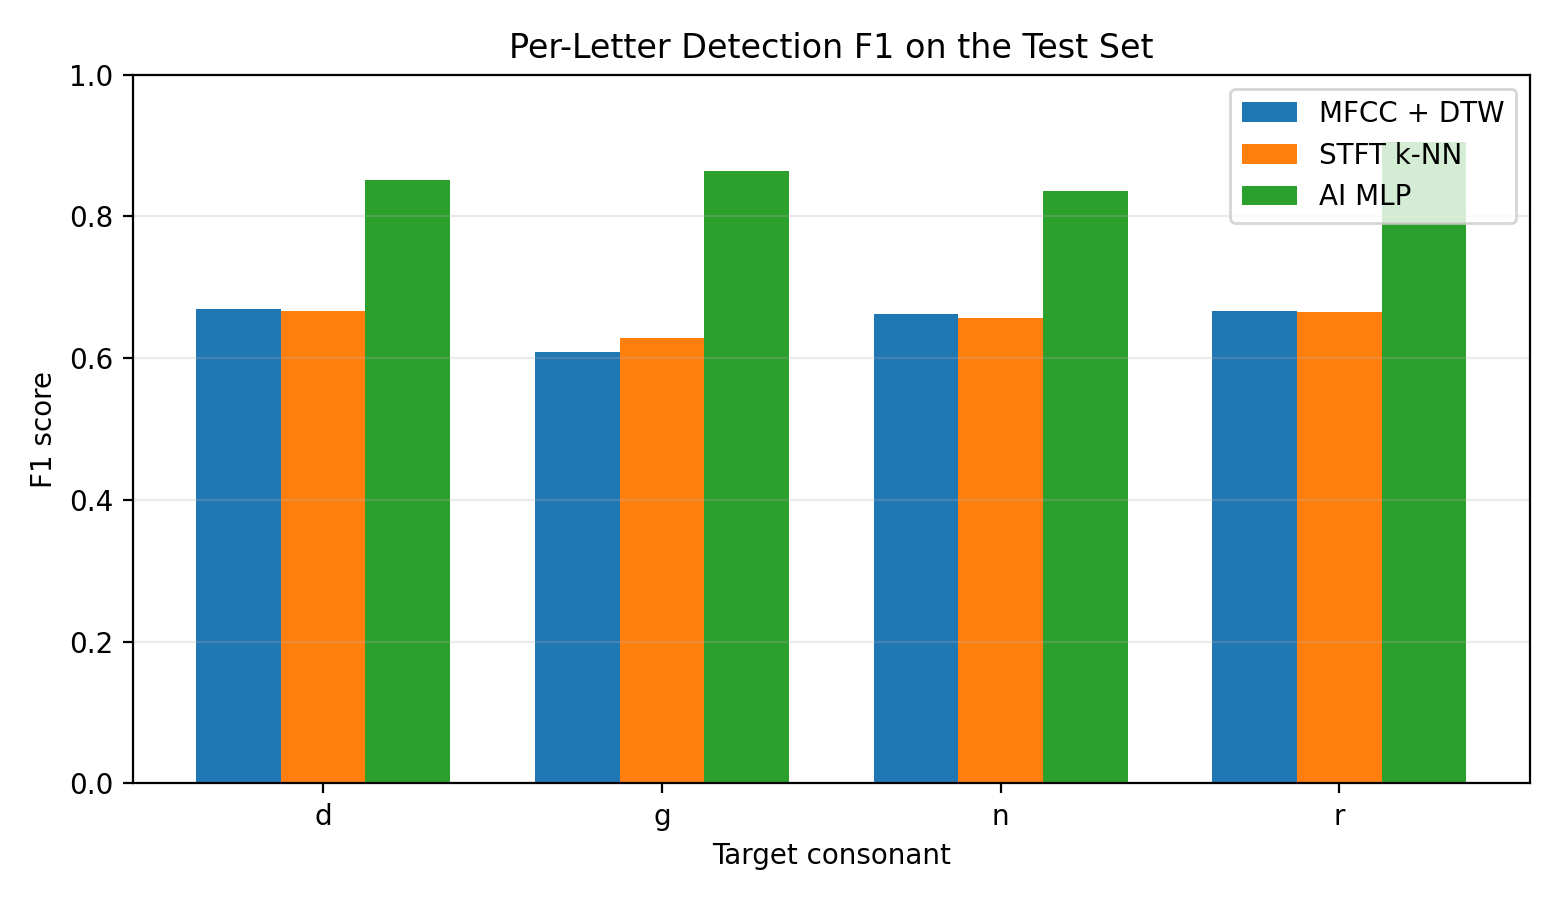
\includegraphics[width=\linewidth]{fullword_per_letter_f1.png}
    \caption{Per-letter detection F1 for an MFCC/DTW baseline, a local-spectrum baseline, and the MLP classifier. Percentage labels are printed above the bars.}
    \label{fig:perletter}
\end{figure}

\subsection{Discussion}
The experiments lead to three main conclusions.

\textbf{1) Weak phoneme alignment is the main bottleneck for classical detectors.}
The classical methods achieve recall around 92--99\%, but precision only around 50--53\%. They often find a spectrally similar local region somewhere in the word, even when the target consonant is absent. This high-recall/low-precision behavior is consistent with positive-template scanning under approximate target localization.

\textbf{2) MFCC/DTW baselines and spectrum baselines are both informative.}
MFCC mean-template and MFCC + DTW represent standard speech-recognition feature and alignment methods. Global FFT, local STFT mean-template, and local STFT k-NN are MATLAB spectrum methods based on direct Fourier analysis. In the full-word setting, none of the classical methods dominates decisively; all are constrained by the same lack of exact phoneme boundaries.

\textbf{3) The MLP gives the highest scores in this study.}
The MLP sees the entire log-Mel representation of the word and learns nonlinear boundaries between positive and negative examples. In the measured results, its macro F1 is 86.25\%, compared with roughly 66--68\% for the classical methods, and its precision and recall are more balanced.

There are still limitations. The target timing is approximate rather than forced-aligned, so the local template banks may include neighboring vowel or transition energy. The balanced design also uses only four positive keyword types per target consonant, which makes the comparison controlled but limits lexical diversity. A phoneme-aligned corpus would allow a cleaner study of purely acoustic consonant spotting, while a larger keyword set would test whether the observed precision gap remains under broader word variation.

\section{Conclusion}
This work analyzed the spectra of four voiced consonants in MATLAB, implemented MATLAB spectrum-based detectors, evaluated MFCC/DTW baselines, and trained an MLP on Speech Commands recordings. The task is formulated as \emph{position-independent} letter detection inside words.

Under that formulation, the five classical detectors all show similar high-recall/low-precision behavior, while the MLP gives the highest measured result with 86.25\% macro F1 and 86.46\% macro accuracy. Overall, Fourier-based spectrum tools remain useful for spectral interpretation and baseline detection, but once target timing becomes uncertain, learned whole-word representations can be more robust than weakly aligned local templates.

\bibliographystyle{IEEEtran}
\bibliography{references}

\end{document}
